\documentclass[french]{article}
\usepackage{graphicx}
\usepackage{caption}
\usepackage[T1]{fontenc}
\usepackage[utf8]{inputenc}
\usepackage{lmodern}
\usepackage{geometry}
\geometry{
	a4paper,
	left=25mm,
	right=25mm,
	top=30mm,
	bottom=30mm,
}
\usepackage{babel}
\usepackage[unicode=true,pdfusetitle,bookmarks=true,bookmarksnumbered=false,bookmarksopen=false,
breaklinks=false,pdfborder={0 0 0},backref=false,colorlinks=true,urlcolor=blue]{hyperref}

\graphicspath{{images/}}

\author{Andrea Brugnoli \\ 
\hspace{2.8pt} Docteur ISAE-Supaéro 2020\\
Ingénieur ISAE-Supaéro 2017}
\title{Méthodes numériques pour la révolution digitale des jumeaux numériques: de la modélisation multi-physique haute fidélité aux modèles réduits pour l'ingénierie}

\date{}

\begin{document}

\maketitle

\large{Dossier de candidature au prix de la fondation Jean-Jacques et Félicia
	Lopez-Loreta pour l’excellence académique}


\begin{figure}[h]
	\centering
	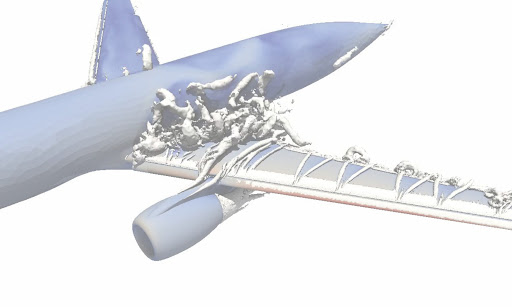
\includegraphics[width=.95\textwidth]{3Dplane.jpg}
	\captionsetup{labelformat=empty}
	\caption{Source: \href{http://www.fenics-hpc.org/}{FEniCS-HPC website}}
\end{figure}





\thispagestyle{empty}

\newpage

\section{Contexte et Objectifs du projet}

\subsection{Le candidat}
La technologie,  les sciences et leur impacte sur l'humaine m'ont toujours intéressé. C'est pour cela que j'ai opté pour un baccalauréat littéraire avec option informatique (obtenu en 2011 a Vérone, Italie). Après mon baccalauréat\footnote{En Italie il est possible d'accéder aux universités scientifique après un Bac. L.}, j'ai obtenu une licence en ingénierie mécanique du Politecnico de Milan. Pendant la première année du master en ingénierie Spatiale, j'ai décide de partir a'l'étranger et j'ai choisi d'effectuer un double diplôme a l'ISAE-Supaéro. J'ai pu approfondir mes connaissances en automatique grâce \`a un master recherche en collaboration avec Supélec/Université Paris Saclay, ainsi que mes compétences en mathématiques appliquées \`a travers un parcours specilis\'e. Mon intérêt pour les systèmes dynamiques et la simulation m'a amené au centre national d'études spatiales (CNES) pour mon stage de fin études, ou j'ai effectué des simulations intensives sur le supercalculateur. \\

J'ai donc décidé de poursuivre un doctorat de recherche dans l'automatique et les mathématiques appliques (calcul numérique), au sein du projet INFIDHEM (Interconnected Infinite-Dimensional Systems for Heterogeneous Media). Le projet consistait a utiliser un formalisme mathématique capable de traiter d'une manière unifiée les problèmes multi-physique. Mon travail était centre sur la modélisation et discrétisation des structures flexibles minces, très utilisées dans l'aéronautique (cf. Fig \ref{fig:IntRod}). Mes travaux de thèse ont été présentés devant un jury international (Thomas Hélie, directeur de Recherches DR2 au CNRS, Yann Le~Gorrec, Professeur ENSMM et Alessandro Macchelli, professeur associé \`a l'Universit\'e de Bologne) et ont été diffuses \`a travers des conférences internationales et 5 articles de revue \cite{brugnoli2019ammmin,brugnoli2019ammkir,brugnoli2020msd,brugnoli2021ther,brugnoli2021num}. \\

Ma forte curiosit\'e pour les thématiques de ma thèse ne m'a pas abbandon\'e dans la suite. C'est pour cela que j'ai décidé de continuer en Post-Doc \`a l'Universit\'e de Twente, dans un projet qui vise a étendre la compréhension de mécanismes physiques sous-jacents le vol biologique (en particulier les oiseux). Mon rôle consiste \`a mettre en place des algorithmes numérique capables de reproduire fidèlement la structure physique du problème \cite{califano2021}.

\begin{figure}[hbt]
	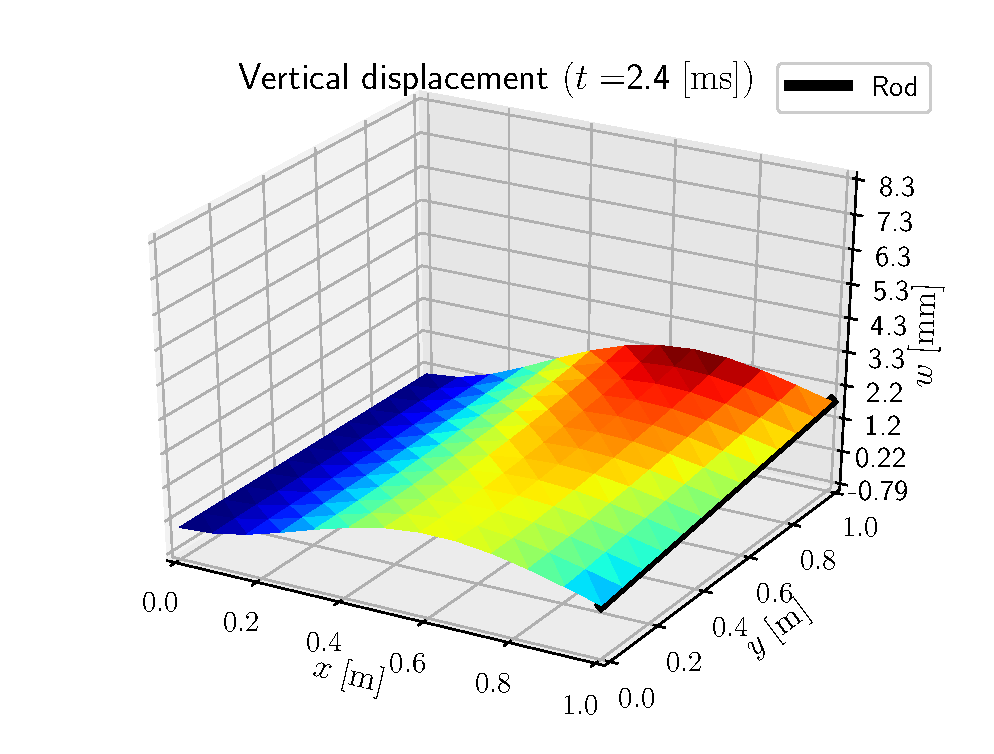
\includegraphics[width=0.5\linewidth]{SnapRod_t25.eps}
	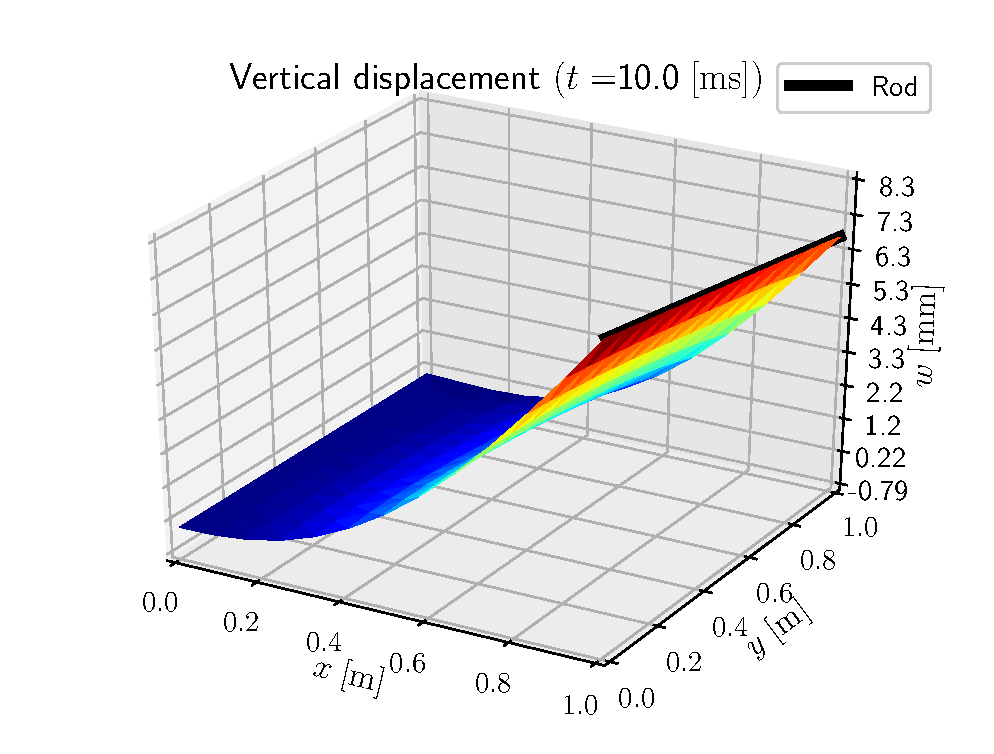
\includegraphics[width=0.5\linewidth]{SnapRod_t100.eps}
	\caption{Simulation d'une plaque mince connectée \`a une poutre rigide.}
	\label{fig:IntRod}
\end{figure}



\subsection{Contexte}

Ma thèse s'est inscrite dans le cadre d'un projet européenne financé par l'agence national de la recherche (ANR) et la Fondation allemande pour la recherche (DFG). L'ambition du projet était de pousser la compréhension d'un formalisme mathématique issu de la physique et de la théorie des systèmes pour le traitement unifié des applications divers (mécanique des solides, des fluides, l'électromagnétisme et la thermodynamique). Il s'agit du formalisme port-Hamiltonien, bas\'e sur la mécanique Hamiltonienne et les graphe de liaisons pour la modélisation des systèmes dynamiques. Il y a 30 ans, le premier article sur cette théorie était publi\`e.  \\

Aujourd'hui ce formalisme a désormais atteint le niveau de maturit\'e pour attaquer problèmes de nature industriel. Il en est convaincu Volker Mehrmann, vice-président de la société mathématique européenne (EMS), qui a illustré les advantages de ce formalisme dans une \href{https://meetings.siam.org/sess/dsp_programsess.cfm?SESSIONCODE=70329}{conférence plénière} a l'occasion de la SIAM Conference on Computational Science and Engineering. Ce niveau de maturit\'e est aussi témoigné par le fait que le conseil de la recherche européen (ERC) \`a récemment attribu\'e \`a \href{https://people.utwente.nl/s.stramigioli?tab=about-me}{Stefano Stramigioli} une subvention de 2.8 millions d'euros pour le projet \href{http://www.portwings.eu/}{Portwings}. Ce projet, dans le quel je suis impliqu\'e pour mon post-doc, cherche \`a améliorer la compréhension du vol battu pour pouvoir perfectionner le design et la construction des robot biomimétiques. L'ambition réside dans le fait d'utiliser la théorie port-Hamiltonien pour expliquer les interactions complexes entre l'aérodynamique et la flexibilit\'e de l'aile (cf. Fig. \ref{fig:pH_view_bird}).

\begin{figure}[tb]
	\centering
	\includegraphics[width = \textwidth]{Bird_Port_Hamiltonian_Subsystems_FULL_ARC.eps}
	\caption{Modèle d'un oiseau robotique bio-inspiré vu comme l'interconnexion de plusieurs systèmes dynamiques. }
	\label{fig:pH_view_bird}
\end{figure}


\subsection{Le projet}
Dans ce projet de recherche, le but consiste \'a mettre en place des méthodes numérique pour accélérer la simulation des problèmes fluide-structure d'un facteur 10-100, par rapport au temps de calcul demandé par une simulation haute-fidélité. Ce projet va donc s'inscrire dans la thématique des jumeaux-numériques. Une éventuelle réussite permettra donc d'intégrer des modèles physique plus économique, qui pourront remplacer des simulations très couteuse et ainsi faciliter le design et la prise des décisions. L'accélération des codes de calcul pour la simulation numérique est considérer un défis fondamental pour faire avancer le niveau technologique de l'industrie aérospatiale (cf. par exemple  \href{https://www.nasa.gov/aero/nasa-issues-a-challenge-to-speed-up-its-supercomputer-code}{NASA Computational challenge} ou \href{https://www.airbus.com/innovation/industry-4-0/digital-design-and-manufacturing-ddms.html}{DDMS}, le programme de digitalisation d'AIRBUS).  \\

Un défis fondamental des modèles réduit est la capacité \`a représenter des physique extrêmement complexes d'une manière précise. 
Dans un premier temps, des simulations haute fidélité seront donc mise en place. Ces modèles numériques devront retenir les propriété physique du problème (conservation d'énergie global, tracement des échanges des énergies entre différents systèmes, conservation d'invariants du problème). Dans un second temps, des technique issus de l'intelligence artificielle seront utilisés pour obtenir des modèles réduit (une technique très prometteuse en ce sens est présentée dans \cite{lee2020}). Dans cette phase, l'impérative reste la fidélité a la physique des modèles ainsi obtenu \cite{willcox2021}. Le dernière objectif consistera \`a utiliser des modèles réduit pour optimiser le design mécanique des structures et vérifier la validité des modèles réduits. 

\section{Organisation du projet}

\subsection{Partenariats académiques}
Pour ce que il concerne la mise en place du projet, des différents partenariat académiques en France et \`a l'international  seront mis en place. Bernhard Maschke (Lyon), Volker Mehrmann (Berlin), Arjan van der Schaft (Groningen) et Stefano Stramigioli (Twente) constitueront les interlocuteur académiques principales. Pour la partie réduction de modèle l'expertise de Charles Poussot-Vassal permettra .... (chercheur principal \`a l'ONERA)

\subsection{Le plan}

\subsection{Budjet}



\footnotesize
\bibliographystyle{unsrt}
\bibliography{biblio_articles}

\end{document}
